% Author: Izaak Neutelings (June, 2018)
\documentclass[border=3pt,tikz]{standalone}
\usepackage{tikz}
\usetikzlibrary{arrows.meta} % to control arrow size
\tikzset{>={Latex[length=4,width=4]}} % for LaTeX arrow head
\usetikzlibrary{calc}
\usepackage{amsmath,bm}
\usepackage{relsize} % for fontsize
\usepackage{xcolor} % for colored text

\colorlet{mylightblue}{blue!5!white}
\colorlet{mydarkblue}{blue!30!black}
\colorlet{myblue}{blue!50!black}
\colorlet{myred}{red!50!black}
\colorlet{mydarkred}{red!30!black}
\colorlet{mydarkgreen}{green!30!black}

\newcommand{\sh}{\kern-0.08em$^\textbf{\#}$\hspace{-3pt}}
\renewcommand{\b}{\kern-0.06em$\flat$}
\renewcommand{\r}[1]{\textcolor{myred}{#1}}

\begin{document}


% FLOW CHART
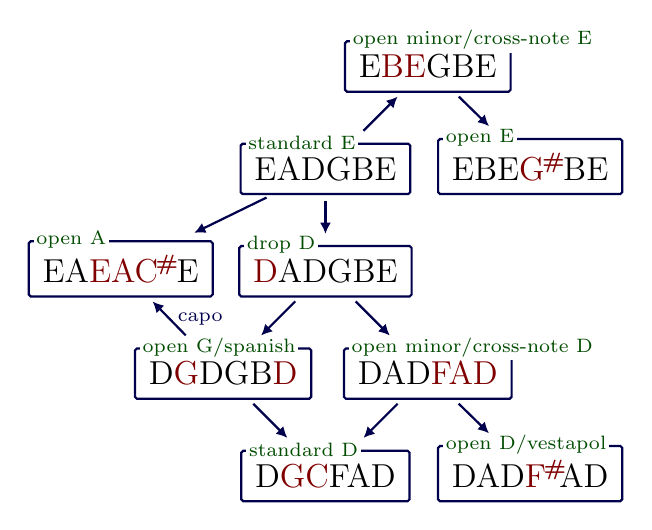
\begin{tikzpicture}[xscale=1.3,yscale=1.3,
                    fscale/.style={font=\relsize{#1}},
                    arrow/.style={->,thick,mydarkblue,shorten <=2,shorten >=4},
                    sarrow/.style={->,thick,mydarkblue,shorten <=2,shorten >=6}]
  \def\c{0.7}
  \def\m{5}
  \def\tuning(#1,#2,#3,#4,#5){
    \node[draw=mydarkblue,thick,rounded corners=\c,inner sep=\m] (#1) at (#2,#3) [fscale=1.2,anchor=south] {#4};
    \node[fill=white,inner sep=1] at (#1.north west) [fscale=-2,right=2,anchor=west,text=mydarkgreen] {#5};
  }
  
  % TUNINGS
%  \tuning(E,  1, 5, EBEGBE,      open minor/cross-note E)
%  \tuning(D,  0, 4, EADGBE,      standard E)
%  \tuning(Dr, 2, 4, EBEG\sh\,BE, open E)
%  \tuning(C,  0, 3, DADGBE,      drop D)
%  \tuning(Cl,-2, 3, EAEAC\sh\,E, open A)
%  \tuning(Cr,2.3,2.9, E\b A\b D\b G\b B\b E\b, standard E\b/half step down)
%  \tuning(Bl,-1, 2, DGDGBD,      open G/spanish)
%  \tuning(Br, 1, 2, DADFAD,      open minor/cross-note D)
%  \tuning(A,  0, 1, DGCFAD,      standard D)
%  \tuning(Ar, 2, 1, DADF\sh AD,  open D/vestapol)
  
  % COLORED TUNINGS
  \tuning(E,  1, 5, E\r{BE}GBE,      open minor/cross-note E)
  \tuning(D,  0, 4, EADGBE,          standard E)
  \tuning(Dr, 2, 4, EBE\r{G\sh}\,BE, open E)
  \tuning(C,  0, 3, \r{D}ADGBE,      drop D)
  \tuning(Cl,-2, 3, EA\r{EAC\sh}\,E, open A)
%  \tuning(Cr,2.3,2.9, E\b A\b D\b G\b B\b E\b, standard E\b/half step down)
  \tuning(Bl,-1, 2, D\r{G}DGB\r{D},  open G/spanish)
  \tuning(Br, 1, 2, DAD\r{FAD},      open minor/cross-note D)
  \tuning(A,  0, 1, D\r{GC}FAD,      standard D)
  \tuning(Ar, 2, 1, DAD\r{F\sh}AD,   open D/vestapol)
  
  % ARROW
  \draw[sarrow,<-] (E)  -- (D);
  \draw[sarrow]    (E)  -- (Dr);
  \draw[arrow]     (D)  -- (C);
  \draw[sarrow]    (D)  -- (Cl);
  %\draw[sarrow]    (D)  -- ([xshift=7]Cr.north west) node[fscale=-2,midway,above=2,right=-2] {capo};
  \draw[sarrow,<-] (Cl) -- (Bl) node[fscale=-2,midway,above=1,right=-2] {capo};
  \draw[sarrow]    (C)  -- (Bl);
  \draw[sarrow]    (C)  -- (Br);
  \draw[sarrow]    (Br) -- (A);
  \draw[sarrow]    (Bl) -- (A);
  \draw[sarrow]    (Br) -- (Ar);
  
\end{tikzpicture}


% CIRCLE OF KEYS
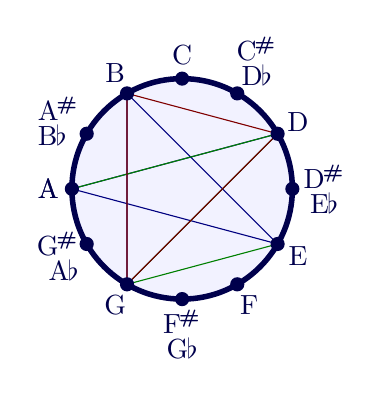
\begin{tikzpicture}[scale=1,
                    %,node/.style={red},
                    dot/.style={draw,circle,inner sep=2pt,fill}]
  \def\R{1.4}
  \def\d{0.3}
  \def\w{2.0}
  \coordinate (O) at (0,0);
  
  % CIRCLE
  \draw[mylightblue,fill] (O) circle (\R);
  \draw[mydarkblue,line width=\w] (O) circle (\R);
  
  % COORDINATES
  \foreach \i/\k [evaluate={\a=(90+(1-\i)*360/12);}]
                 in {1/C,2/Cs,3/D,4/Ds,5/E,6/F,7/Fs,8/G,9/Gs,10/A,11/As,12/B}{
    \coordinate (\k)  at ({\R*cos(\a)},{\R*sin(\a)});
    \coordinate (l\k) at ([shift=({\a:\d})]\k);
  }
  
  % KEYS
  \node[mydarkblue]          at (lC)  {C};
  \node[mydarkblue,above right=-8,align=center]
                             at (lCs) {C\sh\\[-3pt]D\b};
  \node[mydarkblue]          at (lD)  {D};
  \node[mydarkblue,right=-8,align=center]
                             at (lDs) {D\sh\\[-3pt]E\b};
  \node[mydarkblue]          at (lE)  {E};
  \node[mydarkblue]          at (lF)  {F};
  \node[mydarkblue,below=-8,align=center]
                             at (lFs) {F\sh\\[-3pt]G\b};
  \node[mydarkblue]          at (lG)  {G};
  \node[mydarkblue,above=4,below left=-8,align=right]
                             at (lGs) {G\sh\\[-3pt]A\b};
  \node[mydarkblue]          at (lA)  {A};
  \node[mydarkblue,below=4,above left=-8,align=left]
                             at (lAs) {A\sh\\[-3pt]B\b};
  \node[mydarkblue]          at (lA)  {A};
  \node[mydarkblue]          at (lB)  {B};
  
  % TUNINGS
  \draw[blue!50!black]  (E)--(A)--(D)--(G)--(B)--(E);
  \draw[green!50!black] (D)--(A)--(D)--(G)--(G)--(E);
  \draw[red!50!black]   (D)--(G)--(D)--(G)--(B)--(D);
  
  % DOTS
  \foreach \k in {C,Cs,D,Ds,E,F,Fs,G,Gs,A,As,B}
    \fill[mydarkblue] (\k) circle [radius=0.09];
  
\end{tikzpicture}


\end{document}
